% main.tex — Physica A submission, elsarticle class
\documentclass[preprint,12pt]{elsarticle}

\usepackage{graphicx}
\graphicspath{{figures/}}
\usepackage{amsmath,amssymb}
\usepackage{bm}
\usepackage{hyperref}
\usepackage{xcolor}
\usepackage{booktabs}

% shortcuts — consistent with figure notation
\newcommand{\rb}{\rho_b}              % boundary density
\newcommand{\mc}{\mu_\mathrm{c}}      % critical mutation probability
\newcommand{\kavg}{\langle k \rangle} % mean degree
\newcommand{\Lsys}{L}                 % system size
\newcommand{\rmin}{r_{\min}}           % reinforcement threshold
\newcommand{\kmax}{k_{\max}}           % degree cap

\journal{Physica A}

\begin{document}

\begin{frontmatter}

\title{Sharp finite-size coexistence in an adaptive
       multi-species competitive network:
       scaling evidence for a continuous transition}

\author{Evan W. Martin}
\affiliation{organization={Independent researcher}}

% ══════════════════════════════════════════════════════════════════════════════
\begin{abstract}
A three-colour competitive model is studied on a fixed
toroidal lattice and on an adaptive network where edges
co-evolve with node states.
On the fixed lattice the transition is smooth.
On the adaptive network the same local rules produce an
unusually sharp transition: boundary density jumps from
$\rb \approx 0.17$ to $\approx 0.48$ across
$\mu \in [0.35, 0.355]$, distributions are bimodal at
intermediate system sizes ($\Lsys = 128, 256$), and a
variance spike rises four to five orders of magnitude
above the quiet-phase background.
Across $\Lsys = 128 \to 256 \to 384$ the Binder cumulant
dip shallows monotonically toward $2/3$ and the bimodal
window narrows, consistent with a sharp continuous
transition over the tested size range;
a weakly first-order alternative with crossover length
exceeding $\Lsys = 384$ cannot be excluded.
%
A degree-cap sweep ($\kmax \in \{4, 5, 6, 8\}$) implicates
degree headroom as a contributing topological ingredient:
capping at $\kmax = 4$ yields smooth behaviour, while
every $\kmax \geq 5$ yields a sharp jump whose location
drifts toward higher~$\mu$ with increasing headroom.
The headroom reading is partially confounded with a
reinforcement-firing-rate effect (at $\kmax = 4$ the
mean degree falls below the firing threshold) and, in
the local-only control, with candidate-pool shrinkage,
so non-local formation per se is implicated only
indirectly.
\end{abstract}

\end{frontmatter}

% ══════════════════════════════════════════════════════════════════════════════
\section{Introduction}
\label{sec:intro}

Multi-species competition on lattices is a well-studied route to
spatial pattern formation.  Models of cyclic and non-cyclic
competition produce phase transitions between ordered
(species-segregated) and disordered (well-mixed) states whose
universality depends on lattice geometry, number of species,
and the form of the local
dynamics~\cite{szabo2007evolutionary,reichenbach2007mobility,szolnoki2014cyclic}.
On fixed regular lattices, these transitions are typically continuous.

Real populations, however, do not interact on static topologies.
Individuals form and break social, spatial, or ecological links
in response to their own state and the states of their
neighbours---a co-evolutionary feedback between dynamics
\emph{on} the network and dynamics \emph{of} the
network~\cite{gross2008adaptive}.
A growing body of work shows that this feedback can qualitatively
change collective behaviour, including the order of phase
transitions.
Holme and Newman~\cite{holme2006nonequilibrium} and
Vazquez et al.~\cite{vazquez2008generic} demonstrated that
adaptive rewiring converts the continuous fragmentation
transition in the voter model to a discontinuous one.
Gross et al.~\cite{gross2006epidemic} found analogous
sharpening in adaptive epidemic models, and
Demirel et al.~\cite{demirel2011cyclic} studied adaptive
networks with cyclic dominance, showing that coevolution
of topology and strategy leads to spontaneous
network fragmentation.

Here we ask whether topological co-evolution changes the
character of the phase transition in a \emph{conviction-weighted}
multi-species competition model, and if so, what specific
feature of the rewiring drives the change.
Our system differs from prior adaptive-network studies in
three respects:
(i)~node states are continuous three-channel vectors
    (not discrete opinions or strategies), giving a notion
    of ``conviction'' that modulates interaction outcomes;
(ii)~rewiring is globally non-local---new edges may form
    between any two compatible nodes anywhere in the system,
    subject to a degree cap---rather than being restricted to
    neighbours of neighbours;
(iii)~we compare directly against a fixed-lattice control
    to assess the effect of topological freedom.

We find that the same local rules that produce a smooth
transition on the fixed lattice produce an unusually
sharp transition on the adaptive network: a jump in
coupled order parameters, bimodal coexistence visible in
histograms at intermediate system sizes, and a variance
spike.
However, the Binder cumulant dip shallows monotonically
from $\Lsys = 128$ to $\Lsys = 384$, consistent with a
sharp but continuous transition over the tested size range.
A degree-cap sweep ($\kmax \in \{4, 5, 6, 8\}$)
implicates degree headroom as a contributing topological
ingredient, with the jump location drifting monotonically
toward higher~$\mu$ as headroom grows.
The headroom reading is partially confounded with a
reinforcement-firing-rate effect at $\kmax = 4$ and, in
the local-only control, with candidate-pool shrinkage;
non-local formation per se is implicated only indirectly.

The remainder of the paper is organised as follows.
Section~\ref{sec:model} defines the model.
Sections~\ref{sec:fixed} and~\ref{sec:adaptive} present results
on the fixed lattice and adaptive network, respectively,
including control experiments.
Section~\ref{sec:fss} gives finite-size scaling evidence.
Section~\ref{sec:discussion} discusses the mechanism
and connections to related models.

% ══════════════════════════════════════════════════════════════════════════════
\section{Model}
\label{sec:model}

The model is an interacting particle system on an adaptive
network: nodes carry continuous $[0,1]^3$ state vectors,
updates are asynchronous and random-sequential, and in the
adaptive variant the topology co-evolves with the dynamics.
We use ``cellular automaton'' loosely, following the convention
in lattice competition literature.

\subsection{Fixed lattice}

The substrate is an $\Lsys \times \Lsys$ two-dimensional torus:
a square grid with periodic boundary conditions in both directions,
giving every node exactly four neighbours.
This 4-regular toroidal lattice serves as the fixed-topology control.

\subsection{Node state and competition}

Each node~$i$ carries a three-channel colour value
$\bm{c}_i = (r_i, g_i, b_i) \in [0,1]^3$.
The three channels represent three competing species;
the \emph{dominant type} of node~$i$ is the channel
with the largest value.
Ties are broken by a fixed cyclic order $R > G > B > R$.
(This symmetry-breaking is arbitrary; the three species are
otherwise identical, and the phase diagram is symmetric
under relabelling.)
The continuous colour values endow each node with a ``conviction'':
the \emph{dominance margin} is the difference between the
dominant channel and the maximum of the other two.
A node with colour $(0.78, 0.12, 0.04)$ is strongly red
(margin~$0.67$), while $(0.35, 0.33, 0.31)$ is weakly red
(margin~$0.02$) and easily converted.

At each elementary step a node~$i$ is chosen uniformly at random
and interacts with each of its neighbours~$j$.
Channel values change in increments of
$\delta = 1/255 \approx 0.004$:
\begin{itemize}
  \item \textbf{Agreement} (same dominant type):
        both $i$ and~$j$ increment their shared dominant channel
        by~$\delta$ (clamped at~$1$).
  \item \textbf{Conflict} (different dominant types):
        the node with the smaller dominance margin shifts
        toward the winner's type:
        the winner's channel is incremented by~$\delta$ and the
        loser's own dominant channel is decremented by~$\delta$.
        When margins are equal, the focal node~$i$ concedes.
\end{itemize}

A collective reinforcement rule amplifies local consensus:
if at least $\rmin$ of~$i$'s neighbours share the same dominant
type (as determined by the edge relationship after competition),
that channel receives an additional increment.
All experiments use $\rmin = 4$ unless otherwise noted.

One \emph{frame} consists of $N = \Lsys^2$ elementary steps,
corresponding to one sweep of the lattice in expectation.

\subsection{Mutation}

After node~$i$ has interacted with all its neighbours and
reinforcement has been applied, $i$~is reset to a uniformly
random colour---each channel drawn independently and uniformly
from $[0, 1]$---with probability~$\mu$.
Mutation is applied once per node activation, not once per
pairwise interaction.
This mutation is the noise parameter that drives the
phase transition: low~$\mu$ favours local order;
high~$\mu$ disrupts it.

\subsection{Adaptive topology}

The adaptive variant begins from the same 4-regular toroidal
lattice but allows the network to rewire.
After each pairwise interaction between nodes~$i$ and~$j$:
\begin{itemize}
  \item If the edge is \textbf{compatible} (endpoints share
        dominant type after competition): with probability
        $1/N$, a new edge is created between node~$i$ and
        a uniformly random compatible node anywhere in the
        system, provided both endpoints are below the degree
        cap~$\kmax$.
        Up to~8 random candidates are tried; if none qualifies
        (due to degree cap, existing edge, or self-loop),
        the attempt is discarded.
  \item If the edge is \textbf{incompatible} (endpoints differ):
        with probability $1/N$, the edge is severed, provided
        both endpoints retain degree $\geq 2$.
\end{itemize}
The maximum degree is capped at $\kmax = 8$ (twice the
initial lattice degree; the qualitative results are not
sensitive to this choice provided $\kmax$ is moderately
above~4, as it determines the dynamic range of $\kavg$).
The minimum degree floor of~$2$ reduces the frequency of
isolated nodes and extreme fragmentation, but does not
guarantee global connectivity.

Since each of $N$ node activations per frame involves
$O(k)$ pairwise interactions, each with rewiring
probability $1/N$, the expected number of rewiring events
per frame is $O(\kavg)$---of order unity per frame,
scaling with the system.

In the ordered phase ($\mu < \mc$), nodes cluster near
the degree cap: at $\mu = 0.33$, approximately $82\%$ of
nodes have $k = 8$ and $95\%$ have $k \geq 7$.
In the disordered phase ($\mu > \mc$), the distribution
shifts toward the floor: at $\mu = 0.50$, approximately
$44\%$ of nodes have $k = 2$ and $71\%$ have $k \leq 3$.
The degree distribution is thus strongly phase-dependent
(Fig.~\ref{fig:dyn_phase}, Table~\ref{tab:adaptive}).

The result is that ordered regions recruit long-range connections
while disordered boundaries shed them.
The topology and dynamics co-evolve: the network is
simultaneously the arena for competition and a product of it.
A control variant restricts new-edge formation to nodes within
graph distance~2 of the focal node while keeping all other
rules identical (Section~\ref{sec:local_control}).

\subsection{Algorithm summary}

Table~\ref{alg:update} gives the per-node update.
One frame repeats this $N$ times with uniformly random node
selection.

\begin{table}[h]
\centering
\caption{Per-node update for node~$i$.}
\label{alg:update}
\begin{tabular}{@{}r@{\;}l@{}}
\toprule
1. & Snapshot neighbour list $\mathcal{N}(i)$ \\
2. & \textbf{for each} $j \in \mathcal{N}(i)$: \\
3. & \quad \textbf{if} same dominant type: \\
4. & \qquad increment shared channel on both $i$ and $j$ \\
5. & \qquad [adaptive] with prob.\ $1/N$: form edge to random \\
   & \qquad compatible node \\
6. & \quad \textbf{else}: \\
7. & \qquad weaker node shifts one unit toward winner \\
8. & \qquad [adaptive] with prob.\ $1/N$: sever edge $i$--$j$ \\
   & \qquad if both keep degree $\ge 2$ \\
9. & \textbf{Reinforce}: if $\ge \rmin$ edges agree, boost that type \\
10.& \textbf{Mutate}: with prob.\ $\mu$, reset $\bm{c}_i$ to random \\
\bottomrule
\end{tabular}
\end{table}

\subsection{Observables}

The primary order parameter is the \emph{boundary density}
$\rb$: the fraction of edges connecting nodes of different
dominant types.
Low $\rb$ ($\lesssim 0.15$) indicates species-segregated order;
high $\rb$ ($\gtrsim 0.5$) indicates a well-mixed disordered state.

On the adaptive network, the mean degree $\kavg$ serves as a
second, coupled order parameter: $\kavg \approx 7$--$8$ in the
ordered phase (near the cap) and $\kavg \approx 3$--$4$ in the
disordered phase (near the floor).

All reported values are time-averages over the second half of
each run (discarding transients).
Error bars on mean quantities in figures show the standard
error of the mean ($\sigma / \sqrt{n}$) across independent
seeds.
Tables report the seed-to-seed standard deviation~$\sigma$
and population variance.
The primary experiments use 64 seeds; the Binder cumulant
analysis uses 64 seeds per $\mu$ point at every system
size, including $\Lsys = 384$.

\subsection{Note on the reinforcement threshold}

On the fixed 4-regular lattice, $\rmin = 4$ requires all four
neighbours to agree before reinforcement fires---effectively
a unanimity rule.
On the adaptive network, where degree can reach $\kmax = 8$,
the same $\rmin = 4$ requires only half the neighbours to agree.
This asymmetry is inherent to applying a fixed threshold
across variable-degree topologies.
We address its consequences with a control experiment
(Section~\ref{sec:rmin_control}) showing that varying~$\rmin$
on the fixed lattice does not change the transition character.

% ══════════════════════════════════════════════════════════════════════════════
\section{Fixed lattice: smooth transition}
\label{sec:fixed}

On the fixed 4-regular torus ($\Lsys = 128$, 64 seeds,
50\,000 frames), boundary density decreases smoothly with
decreasing mutation probability
(Fig.~\ref{fig:fixed_phase}, Table~\ref{tab:fixed}).
No discontinuity is observed at any $\mu$ tested:
$\rb$ ranges from $0.48$ at $\mu = 0.33$
to $0.08$ at $\mu = 0.10$, with a smooth crossover
near $\mu \approx 0.20$.
This section serves as a baseline: the fixed lattice
transition is smooth, and Section~\ref{sec:adaptive}
asks what changes under adaptive rewiring.

% --- Fixed lattice phase diagram ---
\begin{figure}[t]
  \centering
  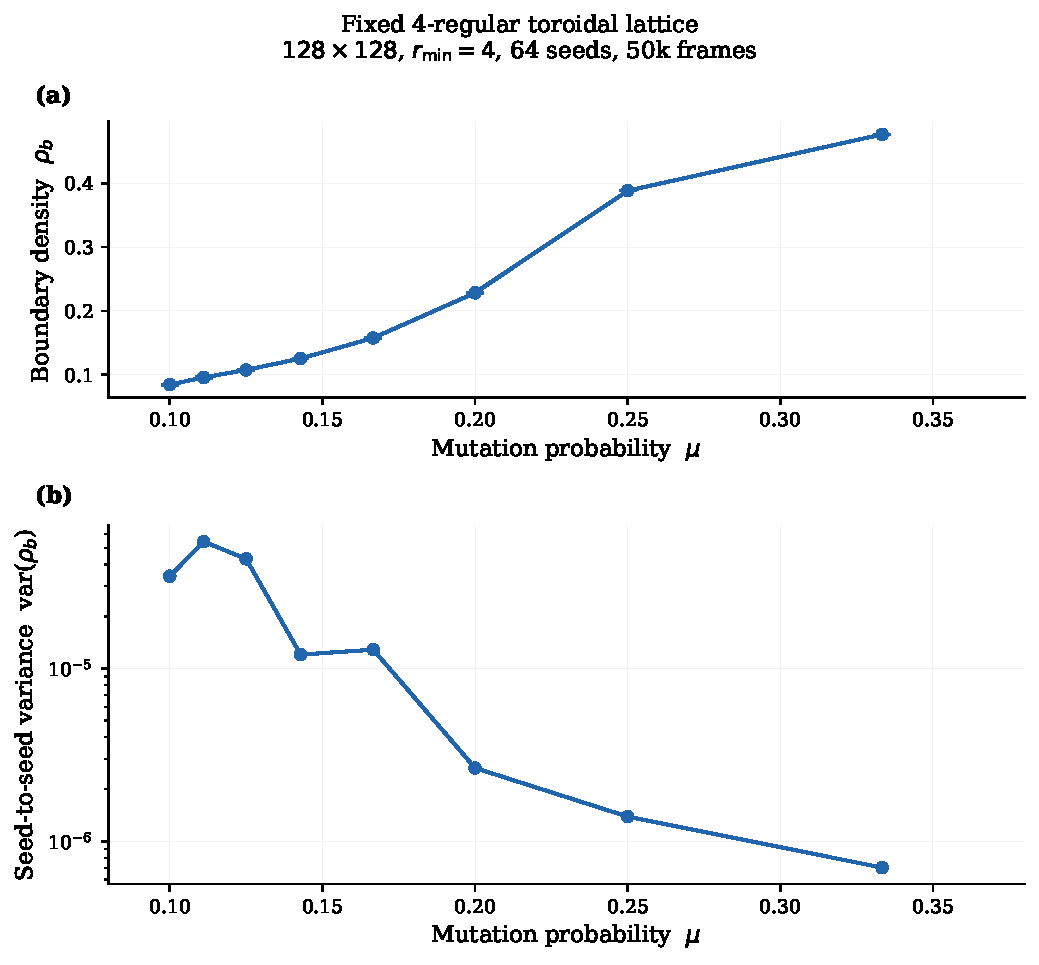
\includegraphics[width=\columnwidth]{fig1_fixed_phase.pdf}
  \caption{%
    \textbf{Fixed lattice phase diagram}
    ($128 \times 128$, $\rmin = 4$, 64 seeds, 50k frames).
    (a)~Mean boundary density $\rb$ vs.\ $\mu$.
    The transition is smooth.
    (b)~Seed-to-seed variance of~$\rb$.
  }
  \label{fig:fixed_phase}
\end{figure}

% Table 1: Fixed lattice phase diagram
\begin{table}[t]
\centering
\caption{Fixed lattice phase diagram ($128{\times}128$, $r_{\min}=4$, 64 seeds, 50k frames).}
\label{tab:fixed}
\begin{tabular}{rrrr}
\toprule
$\mu$ & $\bar{\rho}_b$ & $\sigma(\rho_b)$ & $\mathrm{var}(\rho_b)$ \\
\midrule
0.1000 & 0.0846 & 0.0059 & 3.42e-05 \\
0.1111 & 0.0958 & 0.0074 & 5.42e-05 \\
0.1250 & 0.1076 & 0.0066 & 4.31e-05 \\
0.1429 & 0.1255 & 0.0035 & 1.20e-05 \\
0.1667 & 0.1577 & 0.0036 & 1.29e-05 \\
0.2000 & 0.2284 & 0.0016 & 2.66e-06 \\
0.2500 & 0.3883 & 0.0012 & 1.39e-06 \\
0.3333 & 0.4766 & 0.0008 & 7.04e-07 \\
\bottomrule
\end{tabular}
\end{table}

% Table 2: Adaptive network phase diagram
\begin{table}[t]
\centering
\caption{Adaptive network phase diagram ($128{\times}128$, $r_{\min}=4$, $k_{\max}=8$, 64 seeds, 30k frames).}
\label{tab:adaptive}
\begin{tabular}{rrrrr}
\toprule
$\mu$ & $\bar{\rho}_b$ & $\sigma(\rho_b)$ & $\mathrm{var}(\rho_b)$ & $\langle k \rangle$ \\
\midrule
0.1111 & 0.0270 & 0.0002 & 5.82e-08 & 7.90 \\
0.1250 & 0.0306 & 0.0002 & 5.31e-08 & 7.89 \\
0.1429 & 0.0352 & 0.0002 & 6.23e-08 & 7.88 \\
0.1667 & 0.0418 & 0.0003 & 7.62e-08 & 7.87 \\
0.2000 & 0.0511 & 0.0003 & 1.01e-07 & 7.85 \\
0.2500 & 0.0665 & 0.0004 & 1.26e-07 & 7.80 \\
0.3300 & 0.1016 & 0.0012 & 1.36e-06 & 7.35 \\
0.3333 & 0.1046 & 0.0016 & 2.51e-06 & 7.29 \\
0.3400 & 0.1131 & 0.0034 & 1.18e-05 & 7.06 \\
0.3450 & 0.1257 & 0.0093 & 8.59e-05 & 6.75 \\
0.3500 & 0.1748 & 0.0566 & 3.20e-03 & 5.97 \\
0.3550 & 0.4779 & 0.1230 & 1.51e-02 & 4.21 \\
0.3600 & 0.5483 & 0.0005 & 2.89e-07 & 3.90 \\
0.3700 & 0.5511 & 0.0007 & 4.34e-07 & 3.87 \\
0.4000 & 0.5589 & 0.0007 & 5.03e-07 & 3.79 \\
0.4500 & 0.5706 & 0.0007 & 5.25e-07 & 3.68 \\
0.5000 & 0.5813 & 0.0007 & 5.41e-07 & 3.59 \\
1.0000 & 0.6581 & 0.0006 & 3.66e-07 & 3.12 \\
\bottomrule
\end{tabular}
\end{table}

% Table 3: Initial-condition dependence
\begin{table}[t]
\centering
\caption{Initial-condition dependence across the bistable window ($128{\times}128$, 64 seeds, 30k frames).}
\label{tab:hysteresis}
\begin{tabular}{rlrrr}
\toprule
$\mu$ & Init & $\bar{\rho}_b$ & $\sigma(\rho_b)$ & $\langle k \rangle$ \\
\midrule
0.340 & random & 0.1131 & 0.0034 & 7.06 \\
 & ordered & 0.1133 & 0.0036 & 7.06 \\
\addlinespace
0.345 & random & 0.1257 & 0.0093 & 6.75 \\
 & ordered & 0.1238 & 0.0075 & 6.80 \\
\addlinespace
0.350 & random & 0.1748 & 0.0566 & 5.97 \\
 & ordered & 0.1778 & 0.0515 & 5.95 \\
\addlinespace
0.355 & random & 0.4779 & 0.1230 & 4.21 \\
 & ordered & 0.4458 & 0.1438 & 4.36 \\
\addlinespace
0.360 & random & 0.5483 & 0.0005 & 3.90 \\
 & ordered & 0.5482 & 0.0007 & 3.90 \\
\bottomrule
\end{tabular}
\end{table}

% Table 4: Finite-size scaling at μ=0.35
\begin{table}[t]
\centering
\caption{Finite-size scaling at $\mu = 0.35$ (32 seeds per condition).}
\label{tab:fss}
\begin{tabular}{rlrrr}
\toprule
$L$ & Init & $\bar{\rho}_b$ & $\sigma(\rho_b)$ & $\langle k \rangle$ \\
\midrule
64 & random & 0.1004 & 0.0008 & 7.80 \\
 & ordered & 0.1006 & 0.0009 & 7.80 \\
\addlinespace
128 & random & 0.1819 & 0.0705 & 5.92 \\
 & ordered & 0.1700 & 0.0500 & 6.07 \\
\addlinespace
256 & random & 0.4637 & 0.1151 & 4.21 \\
 & ordered & 0.4517 & 0.1246 & 4.25 \\
\addlinespace
\bottomrule
\end{tabular}
\end{table}



% ══════════════════════════════════════════════════════════════════════════════
\section{Adaptive network: sharp transition}
\label{sec:adaptive}

Allowing edges to co-evolve qualitatively changes the transition.

\subsection{Sharp jump in coupled order parameters}

The phase diagram of the adaptive network
(Fig.~\ref{fig:dyn_phase}, Table~\ref{tab:adaptive}) shows
both order parameters changing sharply between
$\mu = 0.35$ and $\mu = 0.355$.
At $\mu = 0.35$, the majority of seeds converge to the
ordered phase ($\rb \approx 0.17$, $\kavg \approx 6.0$);
at $\mu = 0.355$, most seeds have crossed to the disordered
phase ($\rb \approx 0.48$, $\kavg \approx 4.2$).
By $\mu = 0.36$, all seeds are fully disordered
($\rb = 0.55$, $\kavg = 3.9$).
The boundary density increases by a factor of ${\sim}3\times$
and the mean degree drops by ${\sim}1.5\times$ across this
narrow window.

% --- Adaptive network phase diagram ---
\begin{figure}[t]
  \centering
  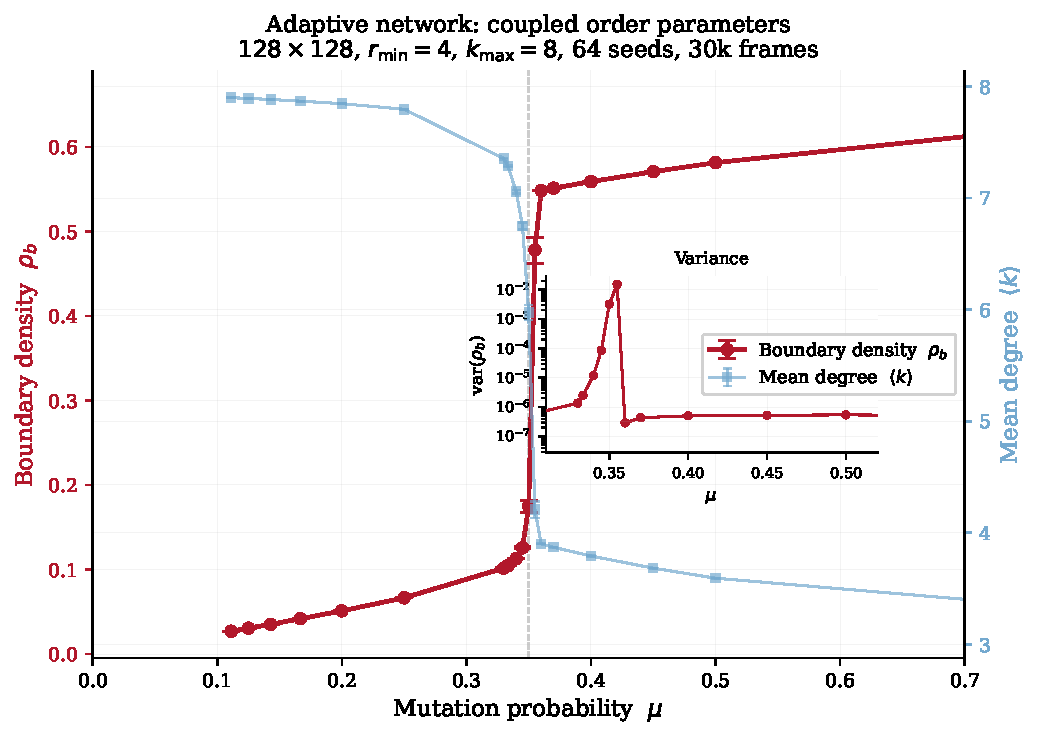
\includegraphics[width=\columnwidth]{fig3_dyn_phase.pdf}
  \caption{%
    \textbf{Adaptive network phase diagram}
    ($128 \times 128$, $\rmin = 4$, $\kmax = 8$, 64 seeds,
    30k frames).
    Boundary density $\rb$ (red, left axis) and mean degree
    $\kavg$ (blue, right axis) vs.\ mutation probability~$\mu$.
    Both order parameters change sharply in the window
    $\mu \in [0.35, 0.355]$.
  }
  \label{fig:dyn_phase}
\end{figure}

\subsection{Topology-independent confirmation and coexistence}

Because $\rb$ and $\kavg$ depend on the edge set, the
sharp jump could in principle be a denominator artifact.
A purely state-based observable, the dominant-species fraction
$f_\mathrm{dom} = \max(n_R, n_G, n_B)/N$
(Fig.~\ref{fig:fdom}), drops sharply from $\approx 0.9$ to
$\approx 1/3$ across the same window, indicating a genuine
state transition rather than a denominator artifact.

% --- f_dom figure ---
\begin{figure}[t]
  \centering
  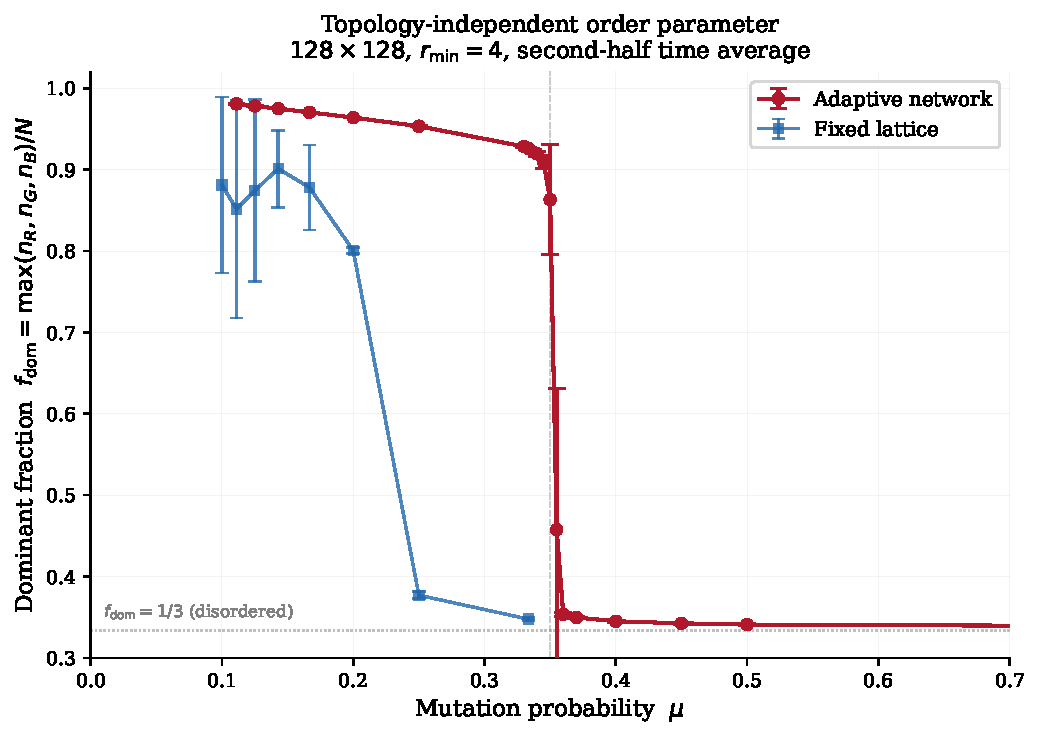
\includegraphics[width=\columnwidth]{fig10_fdom_phase.pdf}
  \caption{%
    \textbf{Topology-independent order parameter.}
    $f_\mathrm{dom}$ vs.\ $\mu$ for the adaptive network
    (red) and fixed lattice (blue).
    The sharp drop indicates that the transition
    reflects a genuine state change.
    Dashed line: $f_\mathrm{dom} = 1/3$ (disordered limit).
  }
  \label{fig:fdom}
\end{figure}

Histograms of per-seed $\rb$ across the transition
(Fig.~\ref{fig:hist_coex}) reveal the distribution shape
more precisely than the scatter plots above.
At $\mu = 0.33$, the distribution is a tight unimodal
peak near $\rb \approx 0.10$.
At $\mu = 0.345$, it remains unimodal but broadens.
At $\mu = 0.35$, the distribution develops a long right tail,
with most seeds near $\rb \approx 0.16$ but a few
reaching $\rb > 0.3$.
At $\mu = 0.355$, the distribution is \emph{clearly bimodal}:
one cluster near $\rb \approx 0.15$ and a second
near $\rb \approx 0.55$, separated by a gap with no seeds.
By $\mu = 0.37$, all seeds have collapsed to a tight
unimodal peak in the disordered phase.

The bimodality at $\mu = 0.355$---with two well-separated
peaks and an empty gap---is the strongest coexistence-like
signature at $\Lsys = 128$.
Section~\ref{sec:binder} shows that these signatures
weaken with increasing system size.

% --- Histogram figure ---
\begin{figure*}[t]
  \centering
  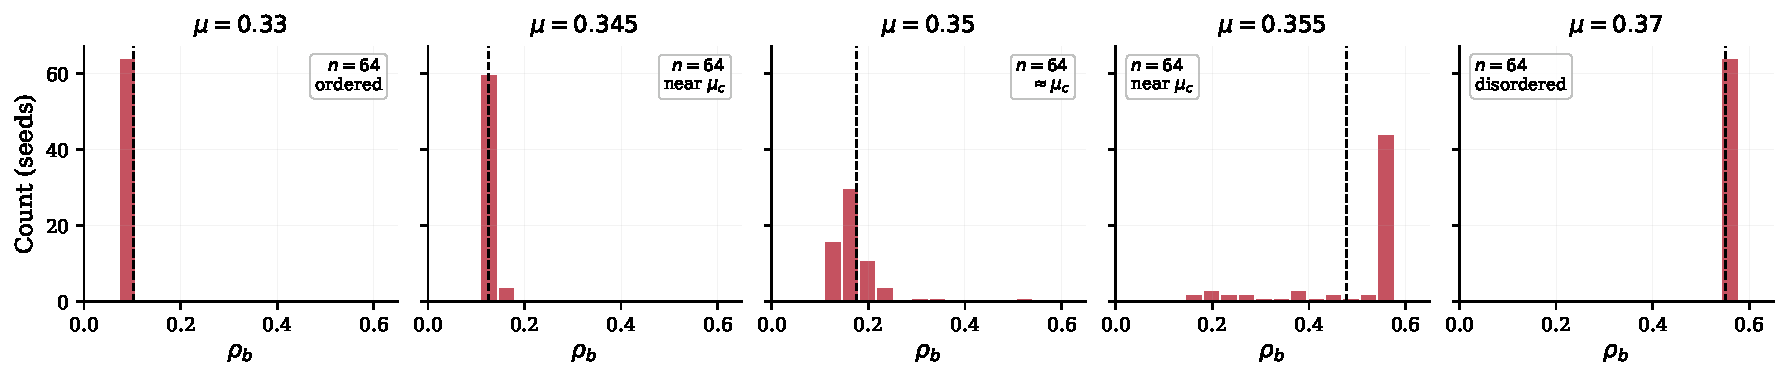
\includegraphics[width=\textwidth]{fig_hist_coexistence.pdf}
  \caption{%
    \textbf{Distribution of per-seed $\rb$ across the transition}
    on the adaptive network
    ($128 \times 128$, 64 seeds, 30k frames).
    At $\mu = 0.355$, the distribution is clearly bimodal
    with an empty gap between ordered and disordered basins.
    Vertical dashed lines mark the mean.
    Some seeds near the transition may undergo basin
    switching during the averaging window (cf.~Sec.~S3).
  }
  \label{fig:hist_coex}
\end{figure*}

\subsection{Variance spike and initial-condition dependence}

The seed-to-seed variance of $\rb$ peaks at
$\mu = 0.355$ with
$\mathrm{var}(\rb) = 1.5 \times 10^{-2}$---four to five
orders of magnitude above the quiet-phase background
(Fig.~\ref{fig:dyn_phase}, inset).

To test for initial-condition dependence, we run at
$\mu = 0.34$, $0.35$, and $0.36$ from both random and
spatially ordered initial conditions
(64 seeds each; Table~\ref{tab:hysteresis}).
At $\mu = 0.34$, both conditions converge to order;
at $\mu = 0.36$, both converge to disorder.
At $\mu = 0.35$, a small fraction of seeds escape to the
opposite basin (3/64 random-init, 2/64 ordered-init),
with means close in both cases
($\bar{\rb} = 0.175$ vs.\ $0.178$).
This is weak initial-condition dependence rather than
strong hysteresis.

\subsection{Controls}
\label{sec:local_control}

To isolate which features of the rewiring drive the
sharpening, we ran two families of controls: a local-only
control restricting new edges to distance-2 neighbours
(all other rules identical), and a degree-cap sweep
varying $\kmax$.

Figure~\ref{fig:threeway} compares four systems at
$\Lsys = 128$ (64 seeds, 30\,000 frames): the fixed lattice,
the local-only adaptive network ($\kmax = 8$), the global
adaptive network with $\kmax = 4$ (matching the fixed-lattice
degree), and the standard global adaptive network with
$\kmax = 8$.

On the local-only network, $\rb$ rises smoothly from
$\approx 0.13$ at $\mu = 0.33$ to $\approx 0.48$ at
$\mu = 0.50$, with no sharp jump at any $\mu$ tested.
The restriction removes the sharp transition, but it also
shrinks the candidate pool from $O(N) \approx 16{,}000$
compatible nodes system-wide to $O(k^2) \approx 50$--$60$
within graph distance~2 at $\kmax = 8$, so it does not
isolate non-locality from formation rate.

A second family of controls varies the degree cap.
At $\kmax = 4$ on the global adaptive network (matching the
fixed-lattice degree), the sharp transition vanishes: $\rb$
rises smoothly from $\approx 0.15$ ($\mu = 0.15$) to
$\approx 0.56$ ($\mu = 0.50$), with seed-to-seed variance
three orders of magnitude below the $\kmax = 8$ case.
Because the network starts at degree~$4 = \kmax$, there is
no headroom for edge accumulation: at initialisation every
node is already at the cap, so formation attempts fail until
severance opens a slot, and mean degree drops monotonically
to $\kavg \approx 3.0$--$3.7$.

To disentangle headroom from outright formation suppression,
we ran intermediate-headroom controls at $\kmax = 5$ and
$\kmax = 6$ (one and two units of headroom respectively).
Both recover a sharp coexistence-like jump
(Fig.~\ref{fig:threeway}):
at $\kmax = 5$, $\rb$ jumps from $\approx 0.20$ at
$\mu = 0.27$ to $\approx 0.51$ at $\mu = 0.30$;
at $\kmax = 6$, the jump shifts to between
$\mu = 0.30$ and $\mu = 0.33$
(from $\rb \approx 0.14$ to $\approx 0.53$);
at $\kmax = 8$, the jump occurs near $\mu \approx 0.345$.
The transition location drifts monotonically toward higher
$\mu$ with increasing headroom.
Over the tested values, the sharp jump is absent at
$\kmax = 4$ and present for $\kmax \geq 5$, suggesting a
threshold-like onset of the sharp coexistence-like
behaviour once some degree headroom is available.

Together with the fixed-lattice baseline and the
local-only control, this $\kmax$ sweep implicates degree
headroom as a contributing topological ingredient:
the sharp behaviour requires some room for like-state
edges to accumulate, but does not require the full
$\kmax = 8$ headroom of the standard setting.
The headroom interpretation is partially confounded
with a reinforcement-firing-rate effect at $\kmax = 4$
(see Section~\ref{sec:mechanism}), and the local-only
control is confounded by candidate-pool shrinkage; an
unconfounded test of either would require an $\rmin$
sweep on the adaptive network or a matched-formation-rate
non-local control respectively, both left to future
work.

% --- Four-way comparison figure ---
\begin{figure}[t]
  \centering
  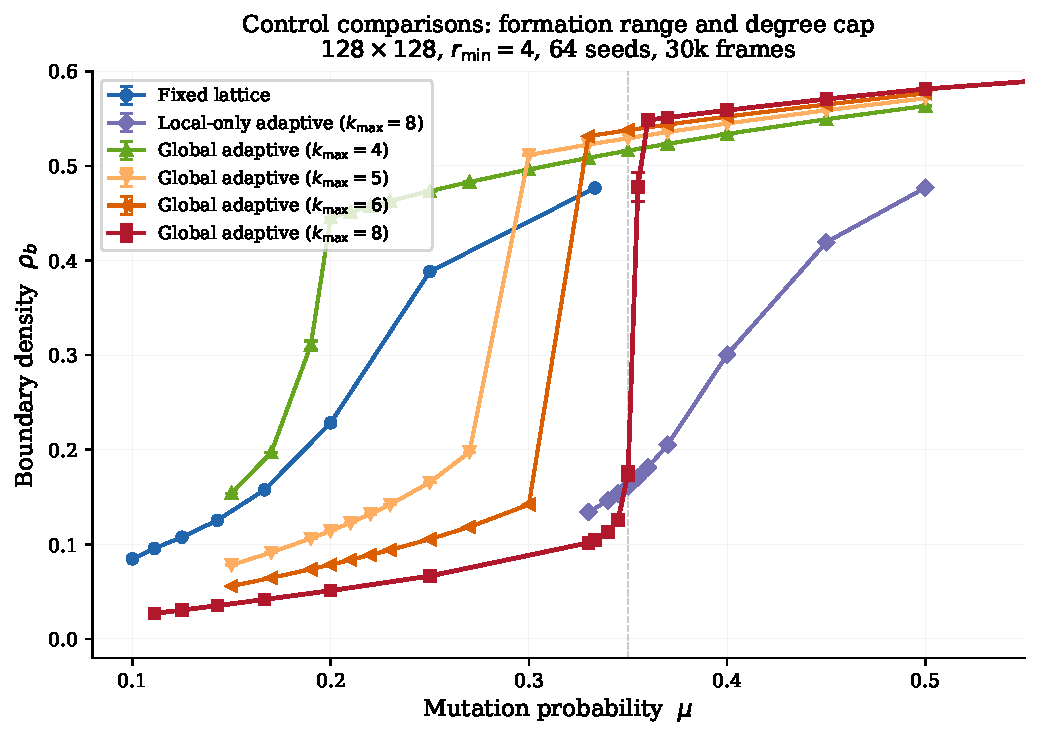
\includegraphics[width=\columnwidth]{fig_threeway.pdf}
  \caption{%
    \textbf{Control comparisons: formation range and degree cap}
    ($128 \times 128$, $\rmin = 4$, 64 seeds, 30k frames).
    Fixed lattice (blue), local-only adaptive with
    $\kmax = 8$ (purple), and global adaptive at four degree
    caps $\kmax \in \{4, 5, 6, 8\}$
    (green, light orange, dark orange, red).
    The sharp coexistence-like jump is absent at
    $\kmax = 4$ but present at every $\kmax \geq 5$;
    the jump location shifts to higher~$\mu$ with
    increasing headroom.
    Caveats: at $\kmax = 4$ the mean ordered-phase degree
    drops below $\rmin$, so reinforcement firing is
    suppressed by construction (see
    Section~\ref{sec:mechanism});
    the local-only control shrinks the candidate pool and
    so does not cleanly isolate non-locality.
  }
  \label{fig:threeway}
\end{figure}

\subsection{Reinforcement-threshold control}
\label{sec:rmin_control}

To rule out an effective-threshold artifact ($\rmin = 4$
is unanimity at degree~4 but only a $50\%$ majority at
degree~8), we repeated the fixed-lattice experiment with
$\rmin = 2$ (64 seeds, 50\,000 frames), matching the
fractional threshold of $\rmin = 4$ at degree~8.
The transition remains smooth and $\rb$ values shift
downward only slightly, making effective-threshold
mismatch unlikely as the explanation.

% ══════════════════════════════════════════════════════════════════════════════
\section{Finite-size scaling}
\label{sec:fss}

We measure $\rb$ at $\mu = 0.35$ for $\Lsys = 64$, $128$,
and~$256$, with both random and ordered initial conditions
(32~seeds each; Table~\ref{tab:fss}).

At $\Lsys = 64$, all 64 seeds converge tightly to the ordered
phase ($\rb \approx 0.10$, $\kavg \approx 7.8$,
combined $\mathrm{var}(\rb) = 7.1 \times 10^{-7}$).
At $\Lsys = 128$, seeds split between basins with
$\mathrm{var}(\rb) = 3.8 \times 10^{-3}$.
At $\Lsys = 256$ (100\,000 frames for equilibration),
most seeds have crossed to the disordered side
($\bar{\rb} \approx 0.46$) but variance remains high
($\mathrm{var}(\rb) = 1.4 \times 10^{-2}$),
indicating that the system is still bistable at this size.

The combined variance \emph{increases} by four orders of
magnitude from $\Lsys = 64$ to $\Lsys = 256$.
At $\mu = 0.35$ the pseudocritical region drifts toward
this value with increasing~$\Lsys$
(Section~\ref{sec:binder}), so part of the variance
increase reflects the approach to the pseudocritical point.
Nonetheless, the strong broadening and bimodal splitting
at $\Lsys = 128$ and $256$ indicate coexistence-like
behaviour at accessible system sizes.

\subsection{Binder cumulant}
\label{sec:binder}

The Binder cumulant
$U_\Lsys = 1 - \langle \rb^4 \rangle /
(3 \langle \rb^2 \rangle^2)$,
where averages are over seeds, provides a standard test
for first-order transitions: $U_\Lsys \to 2/3$ for a
single-peaked distribution, and $U_\Lsys$ develops a
negative dip when the distribution is bimodal.

Figure~\ref{fig:binder} shows $U_\Lsys$ vs.\ $\mu$ for
$\Lsys = 64$, $128$, $256$, and $384$, all with fine
$\mu$ grids ($\Delta\mu = 0.001$; 64 seeds at every
size).
Run lengths scale with system size:
$\Lsys = 64$ and $128$ use 30\,000--50\,000 frames,
$\Lsys = 256$ uses 100\,000 frames, and
$\Lsys = 384$ uses 200\,000 frames---twice as long as
$\Lsys = 256$, partially compensating for slower
equilibration at the largest size.
Spot-checks of $\rb$ time series at $\Lsys = 384$ show
similar within-run basin-switching near $\mc$ to that
documented at $\Lsys = 256$ (Supplementary Material,
Sec.~S3); the doubled run length improves but does not
eliminate this near-critical residence-mixing effect.

The \emph{position} of the minimum shifts to lower~$\mu$
with increasing~$\Lsys$:
$\mu^*(64) \approx 0.360$,
$\mu^*(128) \approx 0.352$,
$\mu^*(256) \approx 0.349$,
$\mu^*(384) \approx 0.348$.
The drift slows with increasing~$\Lsys$, consistent with
convergence toward a finite limiting value, though four
points do not permit a reliable extrapolation.
However, the dip \emph{depth} shallows monotonically
(bootstrap 95\% CI in brackets):
$U_\mathrm{min} = -0.39\;[-0.85, -0.05]$ ($\Lsys = 64$),
$0.26\;[0.18, 0.36]$ ($\Lsys = 128$),
$0.52\;[0.49, 0.55]$ ($\Lsys = 256$),
and $0.58\;[0.56, 0.61]$ ($\Lsys = 384$);
all with 64 seeds.
The confidence intervals do not overlap between
successive sizes from $\Lsys = 128$ onward, consistent
with statistically robust shallowing given the
seed counts.
(At $\Lsys = 64$ the system contains only 4096 nodes and
the deep negative dip may partly reflect small-system
fluctuations; the shallowing trend from $\Lsys = 128$
onward is the more reliable indicator.)
For a standard first-order transition the dip should
deepen without bound as $\Lsys \to \infty$; instead the
minimum recovers steadily toward the single-phase value
$U = 2/3$, consistent with a sharp but \emph{continuous}
transition over the tested size range.
A weakly first-order alternative, in which the Binder
crossover length exceeds $\Lsys = 384$, cannot be
excluded with four sizes; settling the question
definitively would require systems beyond $\Lsys = 384$.

% --- Binder cumulant figure ---
\begin{figure}[t]
  \centering
  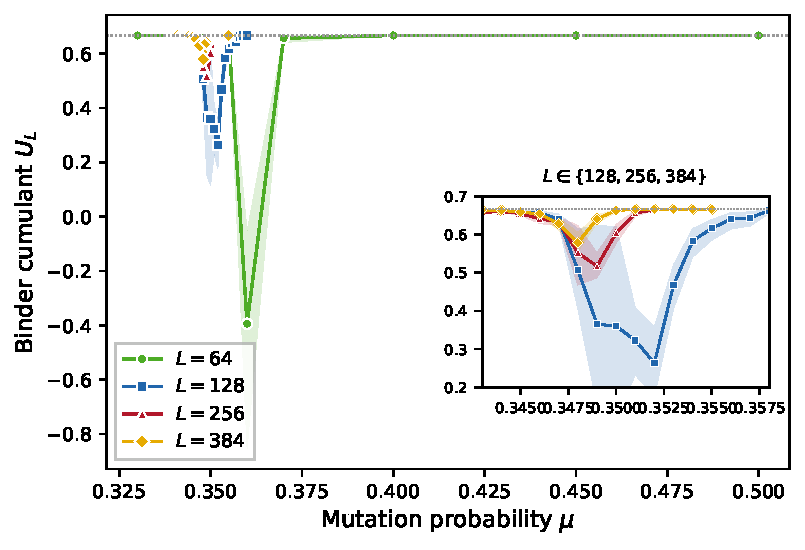
\includegraphics[width=\columnwidth]{fig_binder_sweep.pdf}
  \caption{%
    \textbf{Binder cumulant $U_\Lsys$ vs.\ $\mu$}
    for $\Lsys = 64$, $128$, $256$, and $384$ on the
    adaptive network (fine $\mu$ grids, $\Delta\mu = 0.001$).
    The dip shifts to lower~$\mu$ with
    increasing~$\Lsys$ (pseudocritical drift) and shallows
    monotonically toward $2/3$, consistent with a sharp
    continuous transition over the tested size range.
  }
  \label{fig:binder}
\end{figure}

Per-seed $\rb$ distributions at $\Lsys = 384$
(Supplementary Material, Sec.~S2) show that bimodality
persists at the largest size but is confined to a narrow
window $\mu \in [0.347, 0.349]$ around the Binder
minimum---substantially narrower than the $\Lsys = 128$
bimodal window of Figure~\ref{fig:hist_coex}, consistent
with the same sharpening-yet-continuous trend as the
Binder shallowing.

A two-parameter Binder collapse
$U_\Lsys(\mu) = \tilde{U}((\mu-\mc)\Lsys^{1/\nu})$ does
not succeed for $\Lsys \in \{128, 256, 384\}$:
the $\Lsys = 128$ dip is too deep to be absorbed by any
rescaling, consistent with $\Lsys = 128$ lying outside
the regime where the leading-order finite-size scaling
form holds.
Restricting to $\Lsys \in \{256, 384\}$ yields a tight
collapse, but with only two curves and two free
parameters the exponent is weakly constrained
(bootstrap 95\% CI: $1/\nu \in [0.97, 1.99]$,
spanning standard two-dimensional continuous-transition
exponents without selecting one).
The collapse is therefore consistent with a continuous
transition over the tested sizes but does not assign a
specific universality class;
see Supplementary Material, Sec.~S1
for the full analysis and figure.


% ══════════════════════════════════════════════════════════════════════════════
\section{Discussion}
\label{sec:discussion}

\subsection{Mechanistic interpretation}
\label{sec:mechanism}

The control experiments in Section~\ref{sec:local_control}
narrow the set of topological ingredients that contribute
to the sharp transition.
Sweeping $\kmax \in \{4, 5, 6, 8\}$ shows that any degree
headroom (one unit or more) recovers the sharp
coexistence-like jump, with the jump location shifting
monotonically toward higher~$\mu$ as headroom grows.
The local-only control also restores smoothness but is
confounded by candidate-pool shrinkage from $O(N)$ to
$O(k^2)$ and reduced effective formation rate;
non-local formation per se is implicated only indirectly.
Whether the formation/severance asymmetry contributes
beyond non-local formation alone has not been tested
directly (the converse control, making severance also
non-local, remains future work).

A second confound bounds the headroom interpretation.
At $\kmax = 4$, mean degree in the ordered phase drops to
$\kavg \approx 3.1$, below the reinforcement threshold
$\rmin = 4$; reinforcement firing is therefore
physically suppressed by construction at $\kmax = 4$,
not by absence of a homophily--topology feedback loop
alone.
The $\kmax = 4$ vs.\ $\kmax \geq 5$ contrast partly
reflects this trivial reinforcement-firing-rate effect.
A more interpretable signal is the monotonic $\mu$-shift
of the jump location across $\kmax \in \{5, 6, 8\}$,
where $\kavg \approx 4.8, 5.8, 7.9$ in the ordered phase
(all above $\rmin$) and the jump location moves from
$\mu \approx 0.30$ to $0.345$ with increasing headroom.
The direction of this shift is consistent with the
homophily--topology picture: more headroom yields larger
ordered-phase $\kavg$, so each node experiences more
reinforcement firings per frame in the ordered phase,
making it more robust against mutation and shifting
$\mc$ upward.
Even within the $\kmax \geq 5$ regime the effective ratio
$\rmin/k$ varies from $\approx 0.83$ to $0.51$, so the
shift cannot be cleanly attributed to headroom alone;
a definitive disentanglement would require an
$\rmin$ sweep on the adaptive network at fixed
$\kmax = 8$, which we leave to future work.

The observed behaviour is consistent with a
homophily--topology feedback loop:
in the ordered phase, compatible neighbours accumulate
degree ($\kavg \approx 7$--$8$ at $\kmax = 8$), providing
more reinforcement and competition partners of the same
type and stabilising order against mutation;
in the disordered phase, incompatibility drives edge
severance, lowering $\kavg$ to $\approx 3$--$4$, and
sparse connectivity makes spontaneous ordering difficult.
At intermediate system sizes this loop produces
coexistence-like behaviour in which ordered and
disordered basins are not cleanly separated;
the Binder cumulant trend (Section~\ref{sec:binder})
shows that these signatures weaken at larger~$\Lsys$,
indicating that any effective barrier does not grow
unboundedly with system size.
This picture is qualitatively consistent with prior
adaptive-network results in voter, SIS, and cyclic-dominance
models~\cite{holme2006nonequilibrium,vazquez2008generic,gross2006epidemic,min2017fragmentation,marceau2010adaptive,demirel2011cyclic,durrett2012graph},
where positive feedback between state coherence and
network structure has been identified as a generic
sharpening mechanism.

\subsection{Limitations and future work}

Several aspects of this study would benefit from
further investigation.
Equilibration near $\mc$ remains the principal
technical limitation: time-series spot-checks at both
$\Lsys = 256$ and $\Lsys = 384$ show that some seeds
undergo within-run basin-switching during the
averaging window, so second-half averages near the
Binder minimum partly conflate the two basins
(Supplementary Material, Sec.~S3).
A systematic relaxation-time measurement (frames to
convergence vs.\ $\Lsys$) would clarify this further.

The Binder cumulant dip shallows monotonically from
$\Lsys = 128$ to $\Lsys = 384$, consistent with a
continuous transition over the tested size range.
The two-parameter Binder collapse at
$\Lsys \in \{256, 384\}$ is consistent with standard
two-dimensional continuous-transition exponents but is
weakly constrained by only two curves
(see Supplementary Material, Sec.~S1);
a definitive universality-class assignment would require
simulations at $\Lsys \geq 512$ or
correction-to-scaling fits with additional free
parameters.

The mechanism claim rests on ablation controls, not on
a direct measurement of the feedback loop.
The single highest-value missing control is an $\rmin$
sweep on the adaptive network at fixed $\kmax = 8$, which
would disentangle degree headroom from the
reinforcement-firing-rate effect identified in
Section~\ref{sec:mechanism}.
A matched-formation-rate non-local control and a
non-local-severance control would further sharpen the
roles of formation range and the formation/severance
asymmetry, respectively.
A mean-field theory for the coupled $\rb$--$\kavg$
dynamics would help anchor the simulation results and
predict the location of the bistable window as a function
of model parameters.

% ══════════════════════════════════════════════════════════════════════════════
\section{Conclusion}
\label{sec:conclusion}

On a fixed lattice the three-colour competitive model
shows a smooth transition.
Adaptive non-local rewiring sharpens the transition into
a coexistence-like one with a jump in coupled order
parameters
($\rb: 0.17 \to 0.48$, $\kavg: 6.0 \to 4.2$ across
$\mu \in [0.35, 0.355]$), bimodal histograms at
intermediate system sizes, and a variance spike four to
five orders of magnitude above the quiet-phase
background.
Across $\Lsys = 128 \to 256 \to 384$ the Binder
cumulant dip shallows monotonically and the bimodal
window narrows---consistent with a sharp but continuous
transition over the tested size range, with a weakly
first-order alternative beyond $\Lsys = 384$ not
excluded.
%
A degree-cap sweep ($\kmax \in \{4, 5, 6, 8\}$)
implicates degree headroom as a contributing topological
ingredient, with the jump location drifting monotonically
toward higher~$\mu$ as headroom grows.
The headroom interpretation is partially confounded with
a reinforcement-firing-rate effect at $\kmax = 4$
(mean degree falls below $\rmin$) and, in the
local-only control, with candidate-pool shrinkage;
a definitive disentanglement would require an $\rmin$
sweep on the adaptive network at fixed $\kmax = 8$.

% ══════════════════════════════════════════════════════════════════════════════
\section*{CRediT authorship contribution statement}

\textbf{Evan W. Martin:}
Conceptualization, Methodology, Software, Validation,
Formal analysis, Investigation, Data curation,
Writing -- original draft, Writing -- review \& editing,
Visualization.

\section*{Declaration of competing interest}

The author declares no competing financial interests
or personal relationships that could have appeared to
influence the work reported in this paper.

\section*{Data availability}

The simulation code, raw per-seed data, and analysis
scripts that support the findings of this study are
publicly available at
\url{https://github.com/evanwmart/competitive-ca}.

\section*{Acknowledgments}
The author declares no external funding.
Simulations were performed on personal computing hardware.

\bibliographystyle{elsarticle-num}
\bibliography{refs}

\end{document}
